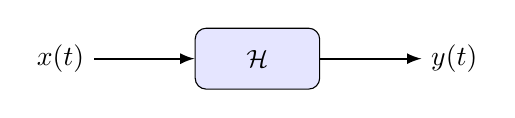
\begin{tikzpicture}[
    auto,
    >=latex,
    block/.style={draw, fill=blue!10, rounded corners, minimum height=2.2em, minimum width=4.5em, font=\small\bfseries},
    sum/.style={draw, fill=blue!10, circle, inner sep=0pt, minimum size=1.5em, font=\bfseries}
]
    \node (tx) at (0,0) {$x(t)$};
    \node[block] (lti) at (2.5,0) {$\mathcal{H}$};
    \node (rx) at (5.0,0) {$y(t)$};
    \draw[->, thick] (tx) -- (lti);
    \draw[->, thick] (lti) -- (rx);
\end{tikzpicture}